
%----------------------------------------------%
% {{{
%----------------------------------------------%

\documentclass[12pt, a4paper, titlepage]{report}
\usepackage[
   margin=2.0cm,
   top=3.5cm,
]{geometry}


%----------------------------------------------%
% Packages
%----------------------------------------------%


\usepackage[utf8]{inputenc}  % Utf-8 input encoding
\usepackage{graphicx}   % Images
\usepackage{float}      % Images floating all around [H]
\usepackage{enumitem}   % Pretty lists (With roman numerals!)
\usepackage{listings}   % Code listings
\usepackage{hyperref}   % Links

% Pretty Captions
\usepackage[format=plain,
            labelfont={bf,it},
            textfont=it]{caption}

% Bibliography
\usepackage[
   style=numeric,
   backend=biber,
   defernumbers=true,
]{biblatex}

% Bibliography Sources
\bibliography{../rc/sources/AITools}   % Remember: no .bib
\bibliography{../rc/sources/manual}
\bibliography{../rc/sources/Maturawork2023}


%----------------------------------------------%
% Metadata
%----------------------------------------------%

\title{RtoV - Deep Learning with Generated Data for Raster Vectorization}
\author{Lars Hoesli}
\date{December 2023}


%----------------------------------------------%
% Macros, commands and definitions
%----------------------------------------------%

% Make title, author and date referable
\makeatletter\let\inserttitle\@title\makeatother
\makeatletter\let\insertauthor\@author\makeatother
\makeatletter\let\insertdate\@date\makeatother

% Make href use italics
\let\oldhref\href
\renewcommand{\href}[2]{\oldhref{#1}{\itshape#2}}


%----------------------------------------------%
% }}}
%----------------------------------------------%


\begin{document}


%----------------------------------------------%
% Title Page and Abstract {{{
%----------------------------------------------%

\begin{titlepage}
    \centering

	 % Title
    \Huge{\textbf{\inserttitle}}
    \par\vspace{0.8cm}
    \LARGE{Matura Work by \insertauthor}\\
    \vspace{0.2cm}
    \large{Supervisor: Beat Temperli}\\
    \vspace{0.2cm}
    \large{\insertdate}
    \vspace{1.5cm}

    % Title picture
    {
       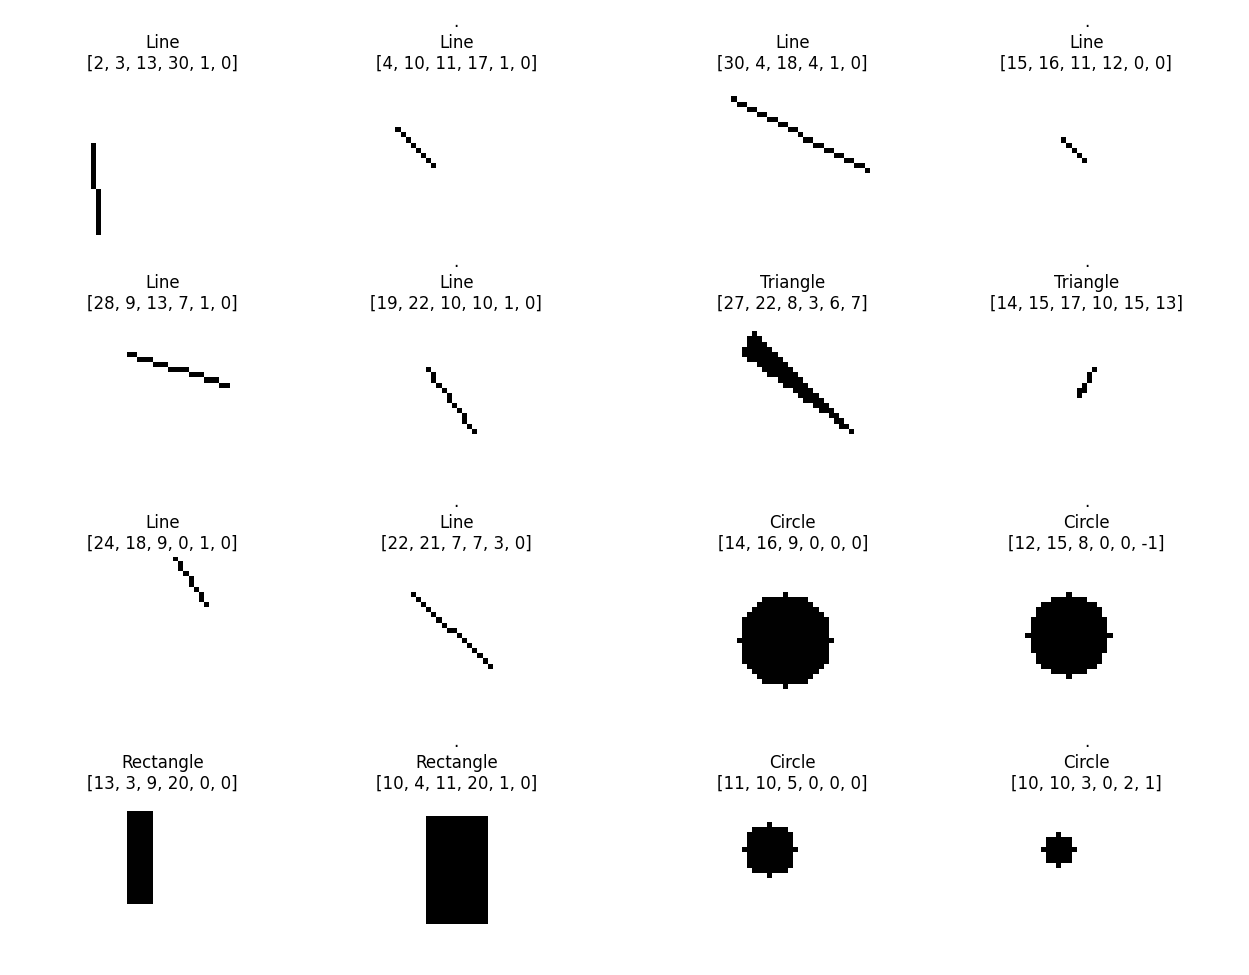
\includegraphics[width=1.0\textwidth]{../rc/images/all_shapes_approx_visual0_condensed.png}
       \label{fig:results_demonstration4_condensed}
    }
    \begin{figure}[ht] % Separate because of the formatting
       \centering
       \caption{An example output of the model used in the demonstration. Two images form a pair, the first being the input image and the second the model output, converted into a raster representation (source \cite{results_demonstration0_condensed})}
    \end{figure}

    \vfill
    % Abstract
    \begin{abstract}
       The conversion from raster images to vector representations remains a challenging task to this day and is actively researched. Due to the inherent difficulties that algorithmic approaches face, such as finding shapes in noisy or blurred images under varying lighting conditions, more research is being done using machine learning, where the most apparent problem is the acquisition of appropriate training data. Therefore, automatically generating pairs of raster images and their corresponding vector representations can be advantageous.
       \vspace{0.3cm}

		 This paper explores this particular approach: Training a machine learning model on generated data pairs. A demonstration is conducted in a limited scope, where a deep learning model is trained on on-the-fly generated data in order to perform the conversion from raster images containing clearly visible shapes into vector representations. The model used in the demonstration is a simple multi-task learning model with a Convolutional Neural Network as a front end and various branches responsible for classifying the shape or determining the features of a particular shape.
       \vspace{0.3cm}

       The model, although trained on a limited number of images, was able to determine the shape with high accuracy and learned to approximate the data relevant for specifying the shapes \emph{Line}, \emph{Rectangle} and \emph{Circle}. The vertices of the shape \emph{Triangle} have proven to be more challenging to estimate and the model presented in the demonstration was not able to provide an accurate representation for this shape.

       \vspace{1cm}
       The code for the demonstration can be found online at \href{https://github.com/lrshsl/RtoV}{github.com/lrshsl/RtoV}
    \end{abstract}

\end{titlepage}

%----------------------------------------------%
% }}}
%----------------------------------------------%

%----------------------------------------------%
% Table of contents {{{
%----------------------------------------------%

\tableofcontents

%----------------------------------------------%
% }}}
%----------------------------------------------%



%----------------------------------------------%
% Introduction {{{
%----------------------------------------------%

\chapter{Introduction}

Images have become an increasingly important part of everyday life, most of which are stored digitally. This makes the search for effective storage of images an essential, well-researched aspect of computer science.
As a consequence, many different formats and compression methods have emerged. The image formats used today can roughly be categorized into two main categories - raster and vector formats.

\section{Raster and Vector Graphics}

Raster and vector graphics are two fundamentally different approaches to representing the content of an image. While raster images store the color values of small parts of a given picture - usually referred to as pixels - to approximate what the image looks like, vector formats store a specification for what shapes can be seen, similar to how humans receive images.

Both methods have pros and cons and are more appropriate for certain situations than others.
Vector formats have numerous advantages for storing images that are easily describable with shapes, especially those consisting of uniformly colored areas or easily describable gradients. To this class of images belong schemes, plots, logos, icons and many more. In these cases, vector graphics can be a more precise and efficient representation of the image than raster formats. A shape described in a vector specification be stored with an infinite resolution, since there are no pixels, while being less storage intensive at the same time. Raster formats, in turn, are better suited for images without easily distinguishable shapes, such as portraits or landcape pictures or photorealistic paintings.

\subsection{Problem Description}

While format conversions among raster or vector and from vector to raster formats is being done by a multitude of programs, the conversion from a raster image to an accurate vector representation proves to be more challenging. This is especially because the shapes and their features seen in the input image have to be recognized in a grid of numbers, which is not an easily solvable problem. Many factors can make it more difficult, such as contrasts in different strengths, noise, and gradients that make it impossible to work with fixed thresholds to detect the contours of shapes. With different manipulations and strategies, such as \emph{hough transform}, \emph{skeletonization} or various edge detection techniques, it is possible to vectorize raster images algorithmically. However, by the time of writing, these approaches are still very limited.

With deep learning, those problems can partially be addressed. The model itself can learn to recognize the shapes in a similar manner as humans do.
However, deep learning models have their own difficulties. For supervised learning, accumulating sufficient training data is a significant challenge and often a limiting factor.

Therefore a way to convert raster images into a vector format is both beneficial and there is no universal solution to it. Deep learning is a powerful tool for this task, especially if the data to train a neural network could be generated indefinitely.
This is why this thesis has been done on the topic of raster-to-vector conversion with deep learning, and focuses on the usage of generated training data to accomplish this task.


\section{Fundamentals}

To understand the concepts and terms used in this paper, a certain basic knowledge of neural networks and deep learning in general is required. In this section, the most relevant information is summarized. This includes general information as well as techniques that are used in the demonstration of this work or mentioned in the discussion. However, it is not meant to be comprehensive and conducting own research is strongly advised.

\subsection{Neural Networks}

Deep learning is done using \emph{neural networks} with several layers of \emph{neurons}. These neurons are connected by \emph{weights} with other neurons.
Each layer of a typical neural network has a \emph{bias value} and an \emph{activation function} associated with it, which are responsible for deciding if a neuron should be activated or not. The network learns through making decisions, which are rated by loss functions. The model is subsequently either punished or rewarded, and its weights are adapted. In that manner, neural networks learn how to accomplish a task through trial and error.

Whilst the bias value is relatively trivial, the various activation and loss functions are important to understand.

\subsection{Activation Functions}

Activation functions are essential components in neural networks that introduce non-linearities. These functions decide whether a neuron should be activated or not based on the weighted sum of its inputs and possibly a bias value if provided.

One widely adopted activation function is the rectified linear unit (ReLU) function.
ReLU, short for rectified linear unit, is a simple yet efficient activation function. Mathematically, it is defined as:
\[ ReLU(x) = \max(0, x) \]
Which is graphically plotted in \ref{fig:relu_function}.

\begin{figure}[h]
   \centering
   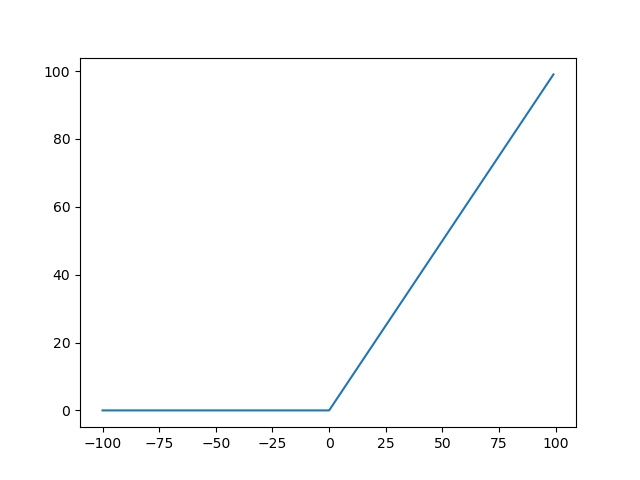
\includegraphics[width=0.5\textwidth]{../rc/images/graph_relu_function.png}
   \caption{ReLU function plotted with $x \in {[-100; 100)}$ (source \cite{graph_relu_function})}
   \label{fig:relu_function}
\end{figure}

In other words, if the input to the ReLU function is negative, it returns zero; otherwise the input value itself is returned. The simplicity of ReLU makes it computationally efficient while still introducing non-linearity. ReLU has become a popular choice in many neural network architectures.

\vspace{0.5cm}
Other popular activation functions include \emph{Softmax}, \emph{Sigmoid}, which squash the input into the range $(0, 1)$ and \emph{Tanh} with a range of $[-1, 1]$.


\subsection{Loss Functions}

Loss functions provide a way to measure the quality of the predictions made by a neural network. Several loss functions exist, each comparing the output of the network with the label. The output usually consists of the values of the neurons in the last layer and is provided as a vector, array or matrix of numbers. The label either already is a vector or similar of the ideal distribution, or is being translated into it.

Loss functions play a crucial role in evaluating the accuracy of the predictions generated by a neural network. They compare the output of the network to the actual values (labels). The output, i. e. the values of the last layer of the network typically takes the form of a vector, array, or matrix. The label may already exist as an ideal distribution in the same form or be translated into one.


One widely used loss function is the \emph{mean squared error} (MSE), which measures the squared difference between the predicted and actual values. The squaring amplifies larger errors while eliminating the sign at the same time:

\[
   MSE(y, \hat{y}) = \frac{1}{n} \sum_{i=1}^{n} (y_i - \hat{y}_i)^2
\]

This is the formula for MSE where $y$ is the true value, $\hat{y}$ is the predicted value and $n$ is the number of samples on which the function is applied.


Another prevalent loss function is \emph{cross-entropy} or \emph{categorical cross-entropy}. They measure the divergence between the predicted probability distribution and the true distribution of labels with the help of the $\log$ function. For categorical cross-entropy the following formula applies:

\[
   CE(y, \hat{y}) = -\sum_{i=1}^{n} y_i \cdot \log(\hat{y}_i)
\]


Minimizing this output of a loss function encourages the output of the model to converge towards the true values and thus improves the accuracy of the neural network.
Some loss functions are better suited for certain tasks than others. The MSE loss is especially suitable for regression tasks, while the CE loss may be a better fit for classification tasks.


\section{Architectures of Neural Networks}

Deep neural networks can be structured in different ways, leading to different kinds of traits that are beneficial in certain situations over others. For raster-to-vector conversion the following architectures are especially interesting.


\subsection{Convolutional Neural Networks}

A convolutional neural network (CNN) is a type of neural network that uses a convolutional layer to extract features from an input image. 

Reducing the information of individual pixels to a sequence of distinct features proves beneficial, as fully connected layers can subsequently learn to establish connections based on these features. In order to extract the relevant features, it uses different \emph{kernels}, which are moved through the images using a certain \emph{stride} value and are applied to the pixel values. A features map is produced. The \emph{kernel} and \emph{stride} values can be adapted to reduce the information for the following layers directly with the convolution layer.
Alternatively, after each convolution, a pooling function can be applied to the feature maps, which reduces the number of features that need to be processed. A usual architecture consists of repeating convolution and pooling layers, which extract the relevant features, and finally fully connected neuronal layers that can logically process the information.

A graphical scheme is shown in figure \ref{fig:cnn_architecture}.

\begin{figure}[h]
	\centering
	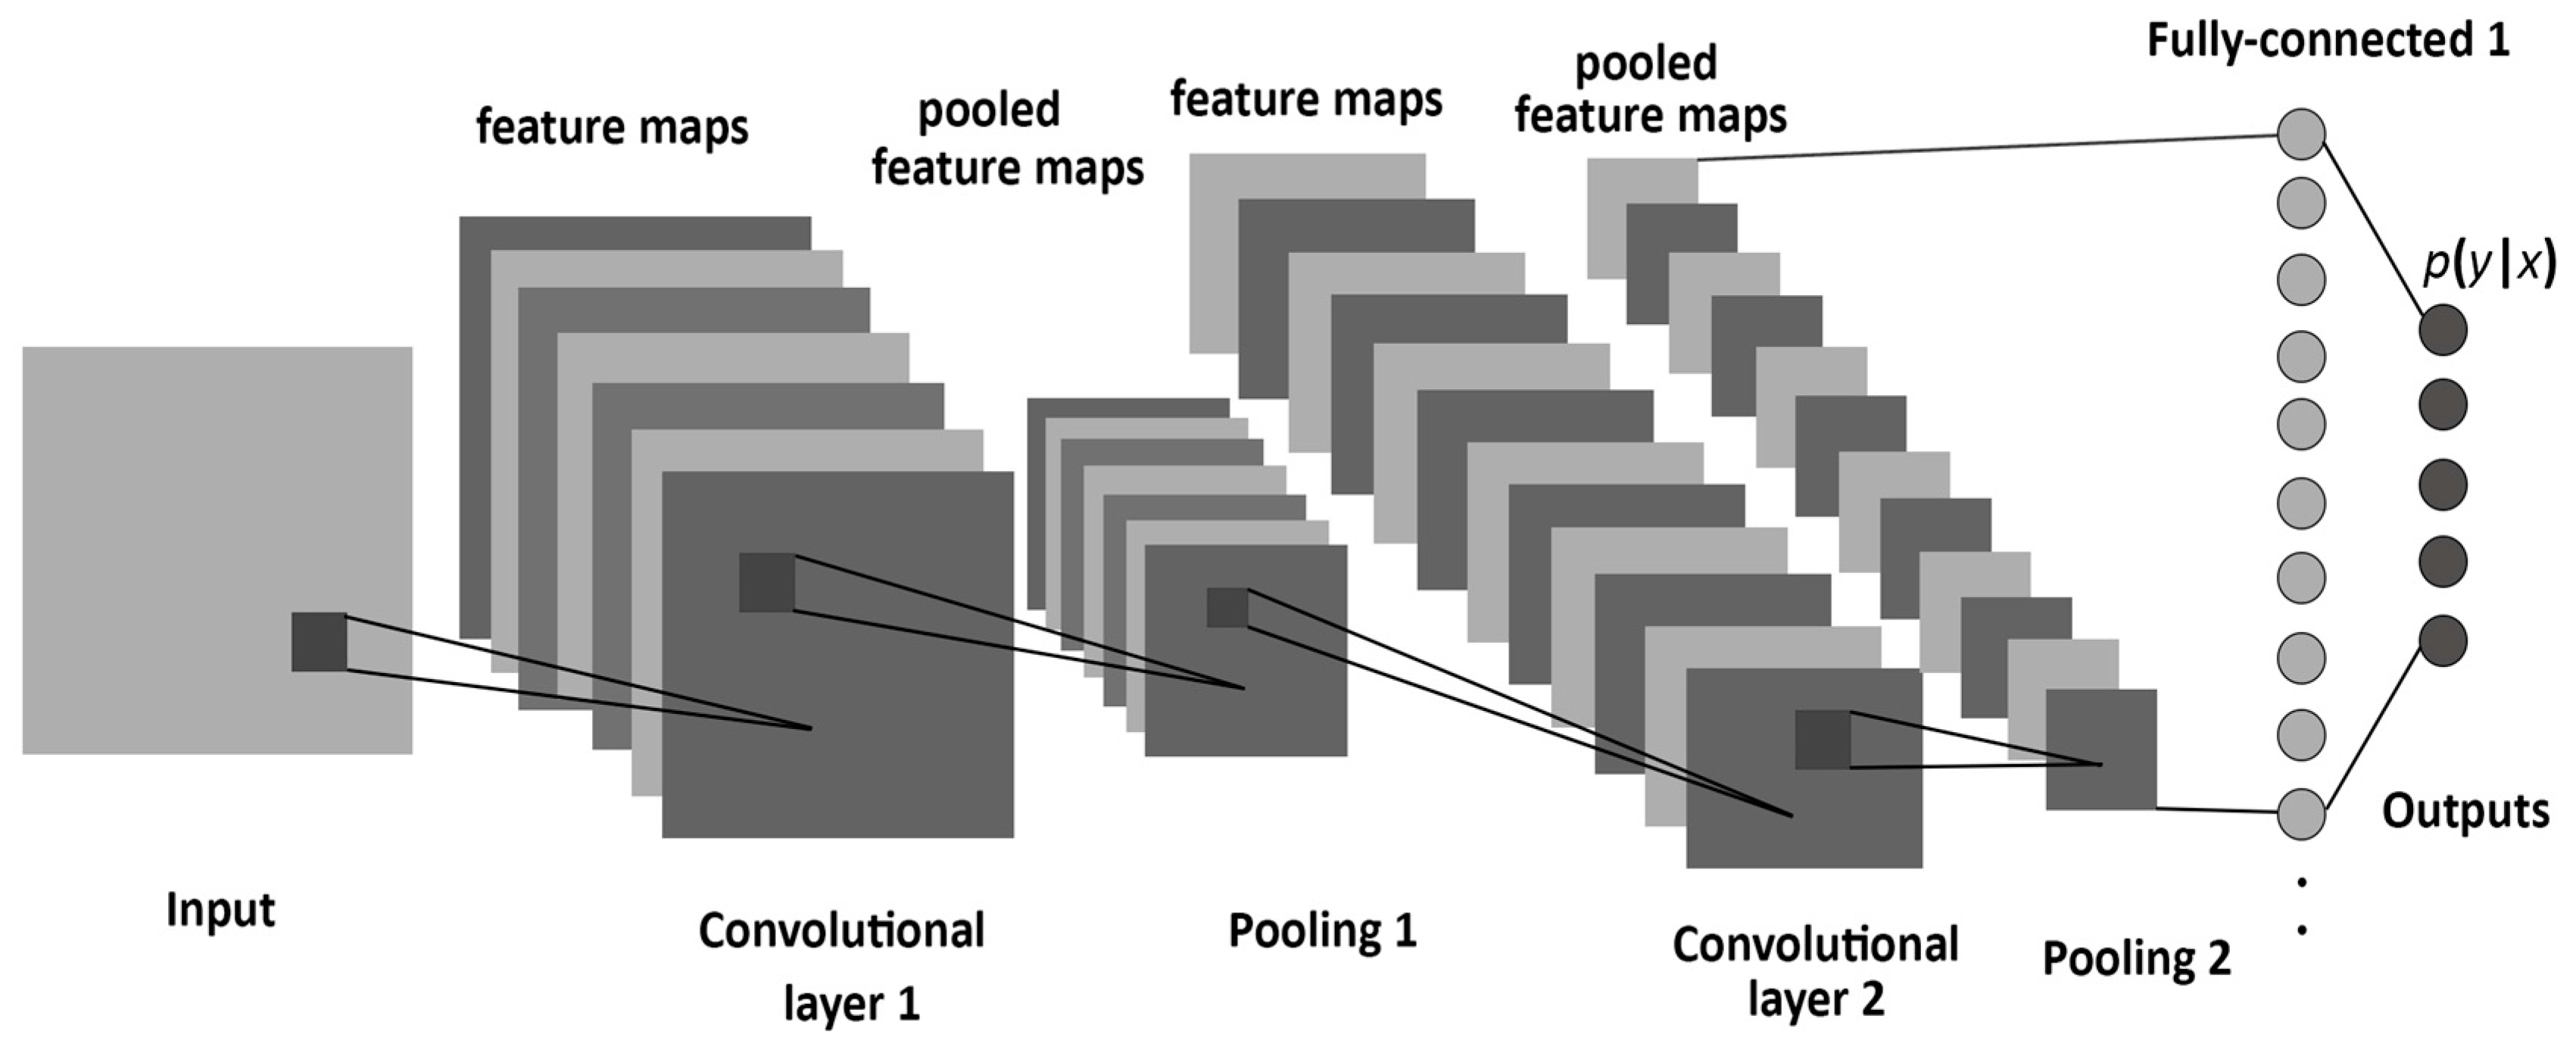
\includegraphics[width=1.0\textwidth]{../rc/images/cnn_architecture.png}
   \caption{Typical Convolutional Neural Network architecture (source \cite{img_cnn_architecture})}
	\label{fig:cnn_architecture}
\end{figure}


Convolutional neural networks poss the ability to automatically identify relevant features in images. As such, they are invaluable for computer vision, object detection, as well as for classification tasks.


\subsection{Recurrent Neural Networks}

Recurrent neural networks (RNNs) are well suited to handle sequential data by remembering information about previous inputs. This kind of memory mechanism is achieved by having loops within the neural network (\ref{fig:rnn_architecture}), allowing Recurrent Neural Networks to retain information and consider past in- and outputs when processing current ones. This makes them ideal for tasks like time series prediction, natural language processing, speech recognition, and more.

\begin{figure}[h]
   \centering
	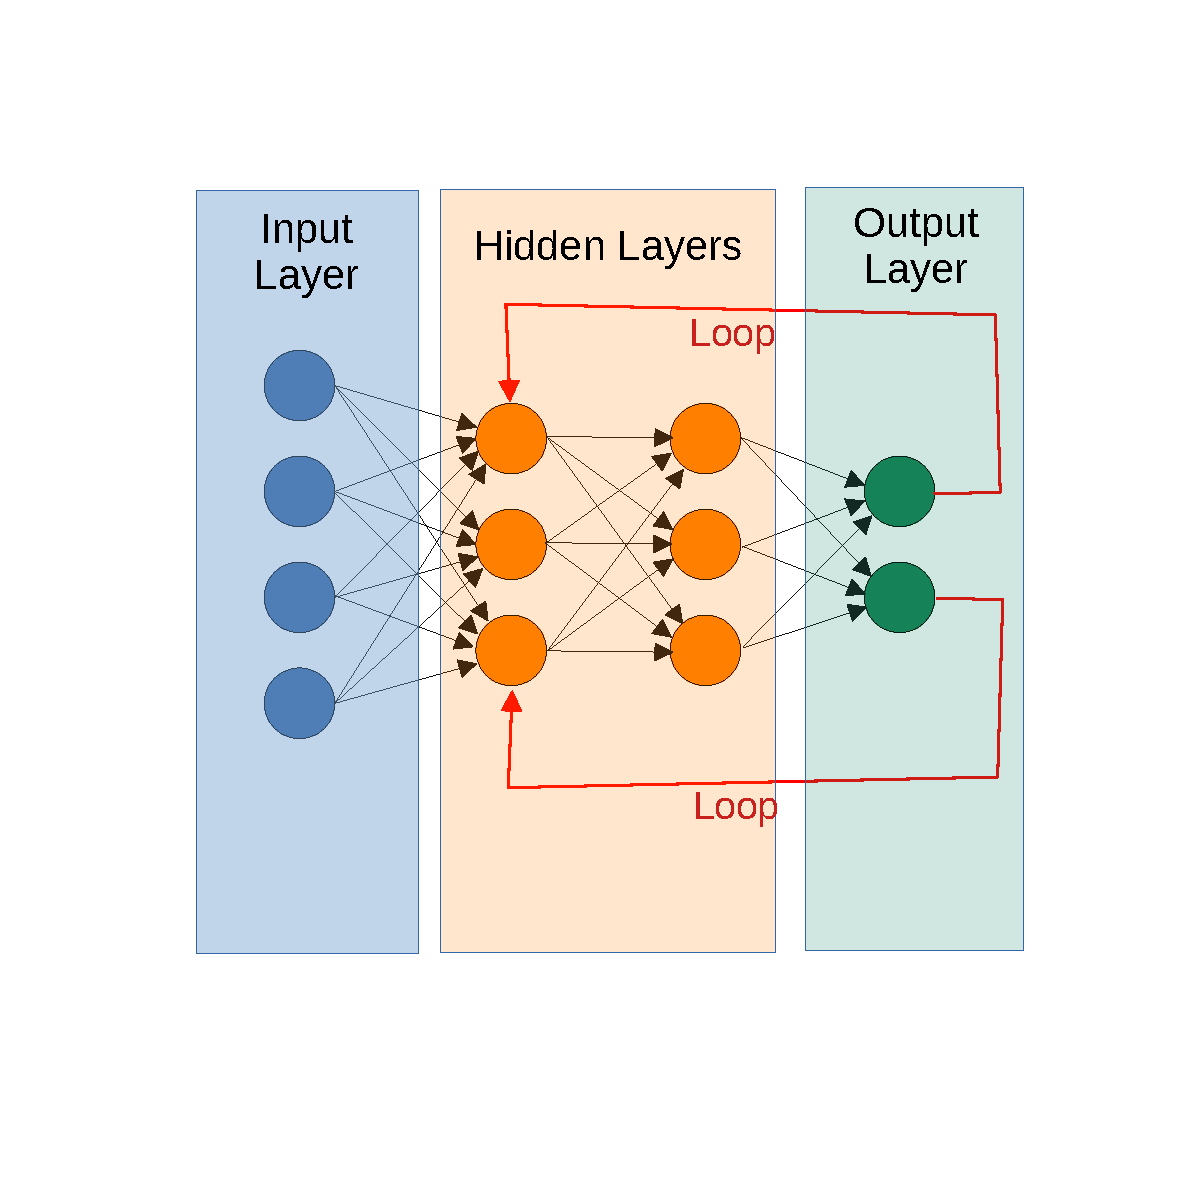
\includegraphics[width=0.6\textwidth]{../rc/images/rnn_architecture.pdf}
   \caption{Example Recurrent neural network architecture (source \cite{img_rnn_architecture})}
	\label{fig:rnn_architecture}
\end{figure}

RNNs have proven valuable in various applications that involve sequential data, allowing machines to comprehend and generate sequences more effectively than standard feed-forward networks. In the case of raster vectorization, this architecture could allow a neural network to remember which shape or vertex has previously been processed, allowing the model to decide which to focus on.

\subsection{Reinforcement Learning}

In Reinforcement Learning (RL), a neural network (\emph{agent}) learns to make decisions by interacting with a given \emph{environment}. This agent makes \emph{actions} in the environment which modify a given \emph{state}. Based on these actions, it receives feedback in the form of rewards or punishments. The goal of the agent is to learn how to maximize the reward.

The agent learns by trial and error, exploring different actions and observing the consequences in terms of rewards. The goal is to discover an optimal policy that leads to the maximum cumulative reward over time. Reinforcement Learning has been successfully applied to various domains, including game playing (e.g., AlphaGo), robotics, finance, and more. They have already proven valuable in raster-to-vector conversion \cite{su_marvel_2023}.

The concept of Reinforcement Learning being very general, a specific use-case for raster-to-vector conversion is presented below. The proposed use of RL for vectorization in this paper is inspired by the work "Marvel - Raster Manga Vectorization via Primitive-wise Deep Reinforcement Learning"  (\cite{su_marvel_2023}).

\begin{enumerate}[label=\Roman*.]
   \item \textbf{Environment}: In the case of the raster-to-vector conversion, the environment is the raster image that is being converted.

   \item \textbf{State}: The state is a copy of the original image, which is modified by the agent each time a new shape is predicted.

   \item \textbf{Action}: The deletion of the shape that was predicted follows as a action that modifies the state.

   \item \textbf{Reward}: The reward is calculated by comparing the original image with the state. To do this comparison, both images would have to be converted into a raster presentation, so that the pixel values can be compared.
\end{enumerate}

\subsection{Multi-Task Learning}

Multi-task learning is an expression used to classify neural networks that solve several related tasks simultaneously in the same model. This allows for some layers or blocks of layers to be reused, and can lead to faster performance than training multiple neural networks separately. It also allows for information to be shared. For instance, the output of one block of layers which might influence which other blocks are used for further processing the information.

Typically, multi-task learning model are used in large neural networks with several common initial layers (here referred to as \emph{front end}). Those layers are often responsible for extracting the relevant data for the subsequent layers. After the front end, the model may split into several independent branches; blocks of layers, specific for separate tasks.

\vspace{0.2cm}
Multi-task learning is advantageous for raster-to-vector conversion. Typically, in raster vectorization, comparatively much time is spent in the initial layers with feature extraction. The information that is extracted in this stage can be used by most if not all subtasks, such as image classification, color extraction and shape approximation. Therefore, it is efficient to reuse the output of these layers for the entire prediction.

%----------------------------------------------%
% }}}
%----------------------------------------------%


%----------------------------------------------%
% Goal and Hypothesis {{{
%----------------------------------------------%

\chapter{Goal and Hypothesis}

A substantial amount of data is needed to train a machine learning model for vectorization of raster images. An ideal data-set would consist of large collections of pairs of raster and vector representations of the same image, which are typically difficult to obtain. Since the conversion of vector images to raster formats is far less difficult, it could be a valid approach to generate random vector images and then convert them into a raster format, to get those raster-vector pairs on which the model can be trained.


This work examines the effectiveness this approach by addressing the following questions:

\begin{enumerate}[label=\Roman*.]
   \item Is it feasible to approach raster-to-vector graphics conversion with a neural network that is trained on randomly generated data?
   \item What strategies or measures have to be taken in order to make this feasible?
   \item What performance can be achieved, and what are the limitations and pitfalls of this approach?
\end{enumerate}


%----------------------------------------------%
% }}}
%----------------------------------------------%


%----------------------------------------------%
% Method {{{
%----------------------------------------------%

\chapter{Method}

\section{Overview}

The training and evaluation data for the model consists of thirty-two on thirty-two pixel images with three color channels, with exactly one shape on each image. The shape is being drawn on all color channels to the pixels that are situated within the shape, resulting in a black shape on a white canvas when plotted.
The generated shapes, as well as their sizes and positions, are randomized and vary with each function call.

\vspace{0.2cm}
The training occurs in several steps:

\begin{enumerate}[label=\Roman*.]
   \item Generation of the training data
   \item Training of the model
   \item Evaluation and adjusting of the model and its weights
\end{enumerate}


\subsection{Shape Generation}

The training and evaluation data in the demonstration consists of white images with a single black shape on them. The shapes are one of the following four: Line, Circle, Rectangle and Triangle. The shapes and their parameters - such as position, size or their single vertices - have been randomized. These features are stored as labels are the basis on which the model is trained.

A function has been developed for the random generation of each shape, returning a numpy array that describes the shape in a numerical representation. This allows it to be compared directly to the output of the model, without an additional conversion step, while representing the relevant features of the image with a minimal number of bytes. Since the number of data points differs from each shape, the array is padded with zeros to match the maximum number of data points. This padding is not being used for determining the performance of the model.

\vspace{0.2cm}
Here is a breakdown of the different shapes and their data representation:

\begin{itemize}
   \item Line: A line is defined through two vertices and width: [x1, y1, x2, y2]. Width and color could be added.
   \item Circle: Center and radius: [x, y, r].
   \item Rectangle: One corner, width and height: [x1, y1, w, h]. A scalar controlling the rotation could be added.
   \item Triangle: Three corner points: [x1, y1, x2, y2, x3, y3].
\end{itemize}

When fully implemented, a color could be included in every shape, taking up four bytes of space, for red, green, blue and alpha channels. In the unmodified demonstration however, the color is not being used since the shape that is being drawn on the raster image is always black.

The function in the current configuration returns a one-dimensional numpy array with a length of six, which corresponds to the number of data points used for a triangle.


The vertices, width and height values generated are constrained to ensure that the shape always remains within the image. However, the possibility that two different shapes can result in the same pixels being colored has not been considered. For instance, a triangle with its corners forming a line may lead to the same input image as a line with the same vertices may produce. In such a case, the model could not possibly know the correct shape and might be punished.

The representation that is obtained after the previous step is written to a numpy array with the shape \lstinline{(100, 100, 3)} or, in graphical terms, a white canvas. To convert from this specific representation to a raster image, a function has been developed (the function \lstinline{draw_on_image} in \lstinline{data/draw_shape_on_image.py}) which accomplishes this task using the \emph{OpenCV2} library.

\subsection{Training}

The training process is structured in epochs, which consist of several batches each. The batch size and the number of epochs are parameterized and can be set by the user, either as flags that are passed to the program or, in the case of the number of epochs, interactively after each training.

The training process on a batch can further be broken down into sub steps:

\begin{enumerate}[label=\Roman*.]
   \item The training images and their labels are generated as explained above and received from the data-loader in a batch
   \item The model processes the images from the batch
   \item The shape loss is computed using the appropriate loss functions
   \item Neural network is being back-propagated with both losses
   \item The losses are recorded for the statistics
\end{enumerate}

The optimizer automatically updates the model according to the back-propagation of the losses. The most important factor for the effectiveness the training is the learning rate, which is a scalar value that determines the impact of the losses on the weights of the model. In the demonstration, no automatic learning rate optimizer is used. However, it can be specified interactively. Through that procedure, the model is trained on all batches.

\subsection{Evaluation}

For the evaluation of the model, its output, which is a numpy array containing a batch of shape predictions and one which contains a batch of the shape specifications is being compared to the ground truth. The shape specifications are numpy arrays with data in the same representation as the one the raster image is generated from.
This is done using the following loss functions: \emph{cross-entropy loss} (CE) for the shape prediction and \emph{mean squared error} (MSE) for the prediction of the data specific to the shape.


\section{Language Choice}  % {{{

Deep learning is a very resource intensive task. Due to time and resource constraints, the language choice was primarily based on the expected development time, but also the flexibility and expected runtime performance of the language and its frameworks and libraries. However, since the computational intensive parts are done within the deep learning library, the availability of performant and established machine learning libraries or frameworks was a higher priority than the performance of the language. A rich and mature ecosystem in general were important as well. On this basis, the table \ref{table:language_evaluation} has been produced, which assigns points to each of the relevant factors. They were mulitiplied by a relevance factor to determine the best fit for the demonstration.
Furthermore, a more in-depth case study of the different languages has been conducted, which provides insight on how the points were selected.

\begin{table}[h]
   \begin{tabular} {|c||p{2.0cm}|p{2.5cm}|p{2.5cm}|p{3.0cm}||p{1.5cm}|}
      \hline
      \textbf{Language}    & \textbf{Perfor-mance} & \textbf{Machine learning libraries} & \textbf{Other ecosystem*} & \textbf{Represent-ative ML Libraries} & \textbf{Rating} \\
      \hline
      Python      & 1 & 5 & 5 & Pytorch, TF        & \textbf{\emph{40}} \\ \hline
      Javascript  & 2 & 4 & 5 & BrainJS, Ml5       & \emph{37} \\ \hline
      C++         & 5 & 3 & 4 & TF, mlpack, CNTK   & \emph{32} \\ \hline
      C           & 5 & 1 & 2 & Darknet, Libtorch  & \emph{16} \\ \hline
      Rust        & 5 & 4 & 3 & Burn, Tangram      & \emph{34} \\ \hline
      Go          & 4 & 3 & 4 & Gorgonia           & \emph{31} \\
      \hline\hline
      \textbf{Relevance} & \textbf{1} & \textbf{5} & \textbf{3} & - & \\
      \hline
   \end{tabular}
   \caption{Language evaluation table\\}
   *The point \emph{Other ecosystem} is rating the availability of libraries that are important for the given task. Namely, libraries for working with raster and vector images and plotting libraries for inspecting the progress of the neural network.

   \label{table:language_evaluation}
\end{table}

\vspace{0.5cm}
{
   \center
   \subsection*{Python}
}
\begin{description}
   \item[Ecosystem] Many well-established and heavily optimized machine learning libraries such as Tensorflow, Keras, Pytorch have been developed for Python. Because of its active community and many libraries, such as \emph{Matplotlib}, \emph{Pandas} or \emph{Pillow}, Python has earned itself the reputation of being the best fit for deep learning and data science.
   \item[Performance] The language performs poorly on benchmark tests \cite{goodmanwen_programming-language-benchmarks-visualization_2023}, but Python libraries are written mostly in C and heavily optimized. Thus, the performance-critical parts are usually fast enough. Performance bottlenecks can also be gradually optimized by switching from Python to Cyphon or directly to C. They are both compiled and can take advantage of type information and are therefore much faster, with little overhead when calling from and into Python.
\end{description}

{
   \center
   \subsection*{Javascript}
}
\begin{description}
   \item[Ecosystem] Many high-level machine learning libraries such as \emph{Brain.js}, \emph{Ml5.js} exist, but few provide the fine-grained control necessary for deep learning research. The ecosystem in general is on a similar level as the one of Python.
   \item[Performance] The language itself usually performs better than Python, but due to its dynamically typed nature, it still is remarkably slower than most statically typed languages.
   \item[Other remarks] Javascript runs in browsers, which would facilitate deployment to the web.
\end{description}

{
   \center
   \subsection*{C++}
}
\begin{description}
   \item[Ecosystem] Many deep learning libraries such as \emph{mlpack}, \emph{caffe} and \emph{Tensorflow} exist. The fast but high-level nature would even allow implementing the machine learning algorithms manually, but since development speed is a priority, this might not be a good choice.
   \item[Performance] C++ is a mature, performant and relatively high-level language. However, the development speed is not optimal. The language focuses on performance over ease of use safety. Much control, but also much responsibility, is given to the developer, which is not advantageous when fast iterations and changes have to be made.
\end{description}

{
   \center
   \subsection*{C}
}
\begin{description}
   \item[Ecosystem] Despite many deep learning frameworks being written in C, they are often designed to be operated from higher-level languages. Machine learning libraries that focus on providing an interface for C like \emph{Darknet} are often very specialized and prioritize speed over ease of use.
   \item[Performance] The language itself belongs to the best performant languages. But the lack of high-level features can slow down development speed. It is also not memory-safe, which can lead to bugs and vulnerabilities.
\end{description}

{
   \center
   \subsection*{Rust}
}
\begin{description}
   \item[Ecosystem] Rust is a promising but relatively new language, and so is its deep learning ecosystem. Comprehensive, performant deep learning frameworks such as \href{https://github.com/Tracel-AI/burn}{Burn} do exist, but are not yet in a stable state and have not yet been able to build up a large ecosystem around it. Calling C functions and thus using C libraries such as \emph{libtorch} is possible, but not an optimal solution.
   \item[Performance] Rust is very performant while still offering high-level features through zero-cost abstractions. As opposed to C++, Rust is also memory-safe due to its built-in borrow checker. It may be the best choice if the deep learning ecosystem was more mature.
\end{description}

{
   \center
   \subsection*{Go}
}
\begin{description}
   \item[Ecosystem] Go is a promising language, but its ecosystem is in a similar state as the one of Rust. Maschine learning libraries like \href{https://github.com/Tracel-AI/gorgonia}{Gorgonia} might soon be as powerful as \emph{Keras}, but have not yet been widely adopted and do not have such a large community behind it as \emph{Tensorflow} or \emph{Pytorch}.
   \item[Performance] Go is faster than both Python and Javascript, and allows to easily add concurrency, which can increase the performance even more.
\end{description}


\subsection{Conclusion}

Python is known to be the most popular or even the best choice for machine learning, due to its various well established libraries and ecosystem. Thus, it has not come as a surprise that the evaluation in this work has come to the same conclusion. Python is a simple language with a large ecosystem and very active community. An advantage that is often not considered is the ability of \emph{Cython}, a Python superset and compiler, to call back and forth into C as well as Python code. This makes an application written in Python or Cython gradually optimizable if needed.

The next best choice might be Rust, but after some experimenting with different libraries, it was decided to stick with Python due to the robustness of its ecosystem. Large parts of Rust's ecosystem are still in an unstable state by the time of this work.

However, the performed evaluation is based on experience and research of the author, as well as common knowledge and is thus not subjective nor comprehensive. It is meant to give an overview of the options and it was tried to make as objective as possible.

% }}}


\section{Framework Choice}

After deciding to write the demonstration in Python, the frameworks had to be evaluated in order to choose the best option. After 

\begin{table}
   \begin{tabular} {|c||p{4.0cm}|p{4.0cm}||p{3.0cm}|}
      \hline
      \textbf{Criteria}          & \textbf{Tensorflow} & \textbf{Pytorch} & \textbf{Project Focus} \\
      \hline
      Written in           & C++ & C & \emph{-} \\ \hline
      Main focus           & Comprehensiveness & Simplicity, fast development in a Pythonic way & \emph{Fast development} \\ \hline
      Ecosystem            & Huge ecosystem with many tools & Comparatively few tools available & \emph{Many good tools} \\ \hline
      Primary application  & Application Production & AI Research & \emph{AI Research} \\ \hline
      Performance          & Highly optimized for large-scale training & Focuses on flexible training and experimentation & \emph{Flexibility, fast iterations and changes} \\ \hline
      Community            & One of the most often used libraries & Often used library & \emph{More often used} \\ \hline
      \hline
   \end{tabular}
   \caption{Framework evaluation table}
   \label{table:framework_evaluation}
\end{table}

\subsection{Conclusion}

After experimenting with both frameworks, \emph{Pytorch} has been chosen for the demonstration. It is a popular and widely used framework and its goals align better with the goals of this work: Simplicity and fast development speed in order to experiment with different architectures is invaluable for this work.
\vspace{0.5cm}

\section{Data Generation}

The data that the model uses for training consists of raster images containing one shape in each. The images are internally represented as numpy arrays, where each entry represents the color values of a pixel. The background is white (i. e. RGB values set to (1, 1, 1)), and the pixels that fall within the shape are set to (0, 0, 0), thus appearing black, so that the contrast between shape and background is maximized.

All data generation is implemented in \lstinline{rtov/data/} and its subdirectories. A class, \lstinline{LazyDataset}, which inherits from the \lstinline{torch.utils.data.Dataset}, provides an interface, which is a Dataloader (\lstinline{torch.utils.data.Dataloader}) object can use later to get the next image. Therefore, the method \lstinline{__getitem__(self, i: int)} is provided, which loads a numpy array, draws a random shape on it and transforms it into a vector.

\section{Model Architecture}

The model in the demonstration is a Convolutional Neural Network, with the usual structure, with several branches as it is typical for multi-task learning. Each branch is a collection of fully connected layers, which can be trained on the output of the front end (i. e. the convolutional and pooling layers).
First, the input image is fed through the convolutional front end: Two blocks with each a convolution layer with ReLU activation followed by a Max Pooling layer. Subsequently, the result is passed through one of the back end that is responsible for the classification of the shape. Depending on the shape that has been predicted in the previous step, the same output of the convolutional layers is passed through another block of fully connected layers which are responsible for the respective shape. Through this mechanism, a conditional form of multi-task learning is achieved, as it is seen in \ref{fig:rtov_architecture}.

\begin{figure}[h]
   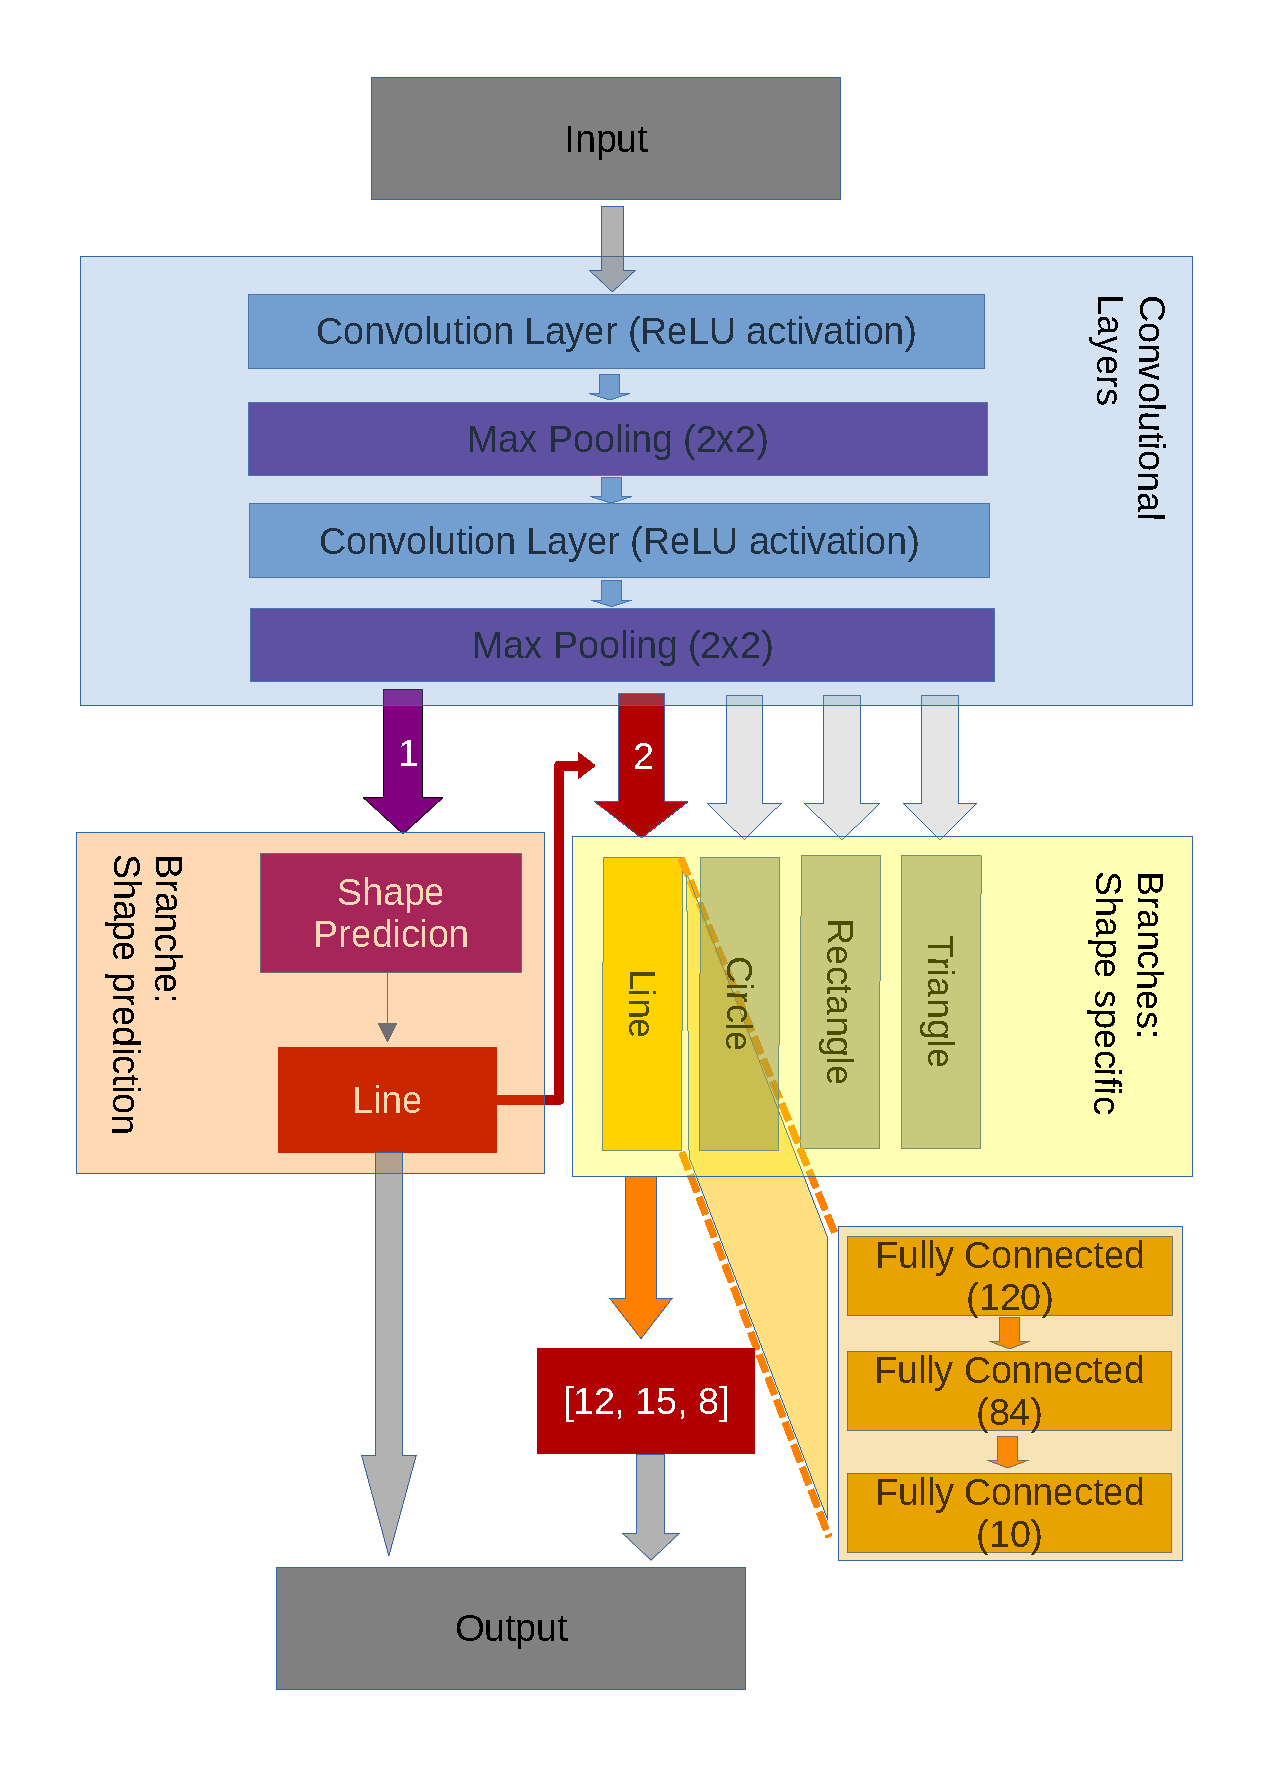
\includegraphics[width=1.0\textwidth]{../rc/images/rtov_architecture.pdf}
   \caption{Model architecture of the demonstration \cite{scheme_rtov_architecture}}
   \label{fig:rtov_architecture}
\end{figure}

%----------------------------------------------%
% }}}
%----------------------------------------------%


%----------------------------------------------%
% Results {{{
%----------------------------------------------%

\chapter{Results}

The model in the demonstration has been able to approximate the shapes it was trained on. The accuracy would need to be improved in order to provide usable results. The given model had problems with approximating triangles; Rather than estimate the positions of the vertices, the model has learned to place those points grouped around the center of the triangle.

Three illustrations are in the appendix for example outputs of the model: Figures \ref{fig:results_demonstration1}, \ref{fig:results_demonstration2} and \ref{fig:results_demonstration3}.
They are rendered in the model evaluation part, obtained through the \emph{test} command in the demonstration.


%----------------------------------------------%
% }}}
%----------------------------------------------%


%----------------------------------------------%
% Discussion {{{
%----------------------------------------------%

\chapter{Discussion}

\section{Results of the Demonstration}

A interesting observation was that the neural network had problems with approximating the shape \emph{triangle}.
There is an explanation for why it was the triangle that the model could not learn to estimate correctly. It is likely due to the nature of the data it needed to extract from the image. What makes the data of the triangle different from the other shapes is that it consisted of three independent vertices, from which the model could have chosen any at any place. The comparison through the MSE loss was not developed enough to determine that a correct vertex prediction but in another order than the label was correct. Thus, the model may not have had the opportunity to make a guess that is rated as correct with a probability higher than $\frac{1}{3}$. The combination of learning rate and this probability might have caused that problem to arise. From the model's point of view, guessing of the real vertices must have not been worth it compared to approximating the center of the triangle. With this strategy, the model tried to minimize the punishment received through the quadratic nature of the MSE loss function.

This seems to be a problem that is very specific for the demonstration and is likely no an inherent issue with the more general approach.

\section{Goals}

The minimal goal has been achieved and the first question has been answered. It is a possible to approximate shapes in a raster image with a vector representation using a neural network that is trained on automatically generated data, as the demonstration has shown. The deep learning model had some difficulties with determining the vertices of triangles. It also could not achieve usable accuracy with the other shapes, but this can be attributed to the time and resource constrains.

This leads to the second question. \emph{What strategies or measures have to be taken to make this [approach] feasible?}
This question could be answered as well. Using a Convolutional Neural Network with multi-task learning was not capable correctly approximating the shapes.

\section{Approach}

The demonstration has been done in a limited scope and does not provide a basis for making general statements about the usage of generated data for raster vectorization.

That being said, The model in the demonstration has shown that a neural network that has been trained on randomly generated raster-vector representation pairs can produce results that resemble the original raster image.
No limiting factors habe been observed that would hinder the scaling of this approach, and there are no apparent reasons for why a neural network with sufficient complexity and training should not be able to perform vectorization of simple raster images.


However, it should to be considered that the data that is used in the demonstration is very limited and has not yet reached a point where it could be used in real world applications. The training and evaluation data consist images containing a single shape, and there are a small number of shapes available. Furthermore, only only data related to the position and size of these shapes. The model outputs a numerical representation of the image, which first would have to be converted into an actual vector format such as SVG.

The demonstration specifically lacks the ability to determine the color of a shape, and cannot be used to convert images containing more than one shape and subsequently never learned how to recognize relations between the shapes in an image.

\vspace{0.5cm}
Those are limitations of demonstration and not necessarily of the approach itself. The model used in the demonstration cannot answer the question of whether those obstacles can be overcome or not.

Those observations could be made:

\begin{enumerate}[label=\Roman*.]
   \item Even a model trained on a CPU can quickly learn to extract shapes from raster images using the generated data.
   \item To scale and improve the model, many optimizations could still be taken in the sections model architecture, training data and training parameter optimization.
   \item No obstacles have been observed when increasing the complexity of the training data. There is no apparent reason why it should not be possible to make a model learn more complex data.
   \item A more sophisticated model may be needed for further experiments.
\end{enumerate}



\section{Proposed Model Architecture}

There are various strategies and architectures for converting raster images to vector images using deep learning. Based on the experience gained during the progress of this work, an architecture is proposed for projects extending beyond this thesis. A comprehensive structure is given that incorporates elements from various deep learning strategies, combining Recurrent Convolutional Networks with Reinforcement Learning while keeping the multi-task learning nature used in the demonstration.

\begin{enumerate}[label=\Roman*.]
   \item A random array of numbers is generated, which describe the image and its shapes in a vector-like format.
   \item The input is a raster image represented as an array.
   \item The first layers are convolution and pooling layers. They are applied directly to the input image to extract the relevant features.
   \item The output of the convolutional layers is directly passed to one or more small, independent fully connected layers. These layers are used to classify the shape as well as the color of the shape and background. A separate CNN might be useful for those layers, but this has to be investigated further. Here, the model could incorporate features from Residual Neural Networks, such that the output of the first CNN layers is directly passed to following layers, without going through the entire CNN block.
   \item Afterwards, the output of the CNN layers is passed to another set of fully connected layers, which are specific for the shape that has already been predicted. These layers are used to extract the shape-specific data, such as position, rotation, corner points or size.
   \item The output is then converted into a raster format, which then is compared to the input image

   \item For the loss function two fundamentally different approaches are considered:
      \begin{itemize}
         \item Comparing the output of the model directly with the label. This approach is used in the demonstration and is computationally very efficient.
         \item Converting the output, together with the previous predictions, into a raster image, and comparing it to the input image. This could lead to more precise results and provides more meaningful feedback to the model.
      \end{itemize}

   \item Recurrent capabilities can be incorporated:
      \begin{itemize}
         \item Long term memory, in order to make the model remember which shapes have already been predicted. This could help the model to learn relations between the shapes in a given image. However, using reinforcement learning would facilitate this further, since this information can be stored in the \emph{state}.
         \item Short term memory can be very advantageous in the shape-specific layers. This could resolve the difficulties the model had with approximating the vertices of triangles in the demonstration.
      \end{itemize}
\end{enumerate}


\pagebreak
\section{Conclusion}

The demonstration and research have shown that deep learning with generated vector-raster image pairs can be a useful technique for raster vectorization, at least in the first stage of training a neural network. The generation of the random images helps to obtain valuable labeled image pairs.
However, the demonstration has shown that approximating a raster image in a vector format remains a challenging task even with an infinite amount of training data available. The model in the demonstration has been able to learn how to classify the four shapes, and could extract the relevant information to roughly approximate most of them; triangles have proven more challenging.

Furthermore, an architecture has been proposed that might be able to leverage the advantages of various deep learning architectures and techniques, which could address those challenges. It might be a starting point for future works, and successfully implementing such a neural network and training process might as well result in an efficient way to vectorize raster images in practical applications.


%----------------------------------------------%
% }}}
%----------------------------------------------%


%----------------------------------------------%
% Bibliography {{{
%----------------------------------------------%

\chapter{Sources and References}

\nocite{*}  % Show all bibliography entries

% Text Resources
\begin{refcontext}[labelprefix=T]
   \printbibliography[type=misc, keyword={TextResource}, title={Text Sources and References}]
\end{refcontext}

% Image Resources
\begin{refcontext}[labelprefix=I]
  \printbibliography[type=misc, keyword={ImageResource}, title={Image Resources}]
\end{refcontext}

% AI Tools used
\begin{refcontext}[labelprefix=A]
   \printbibliography[type=misc, keyword={AITool}, title={AI Tools}]
\end{refcontext}

%----------------------------------------------%
% }}}
%----------------------------------------------%

%----------------------------------------------%
% Appendix {{{
%----------------------------------------------%

\chapter{Appendix}

\begin{description}
   \item[Code] The code for the model can be found at the following link or when scanning the QR-Code below: \href{https://github.com/lrshsl/rtov.git}{github.com/lrshsl/RtoV}
   \item[This Paper] This paper is available as a PDF and latex file at \href{https://github.com/lrshsl/matura-doc/tree/main/matura_thesis}{github.com/lrshsl/matura-doc}
\end{description}


\begin{figure}[b]
   \centering
   
\includegraphics{../rc/images/QrCode_LinkRepo.png}
   \caption{Link to the github repository with the code for the demonstration}
\end{figure}

\pagebreak

The following illustrations are example outputs of the \emph{test} command of the demonstration. Two images each form a pair, the right one of which is the original raster representation, the left is the output of the model when evaluated on the right image. The model output has been converted into a raster format. The exact numerical data is shown above the respective image.
\vspace{2cm}

\begin{figure}[H]
   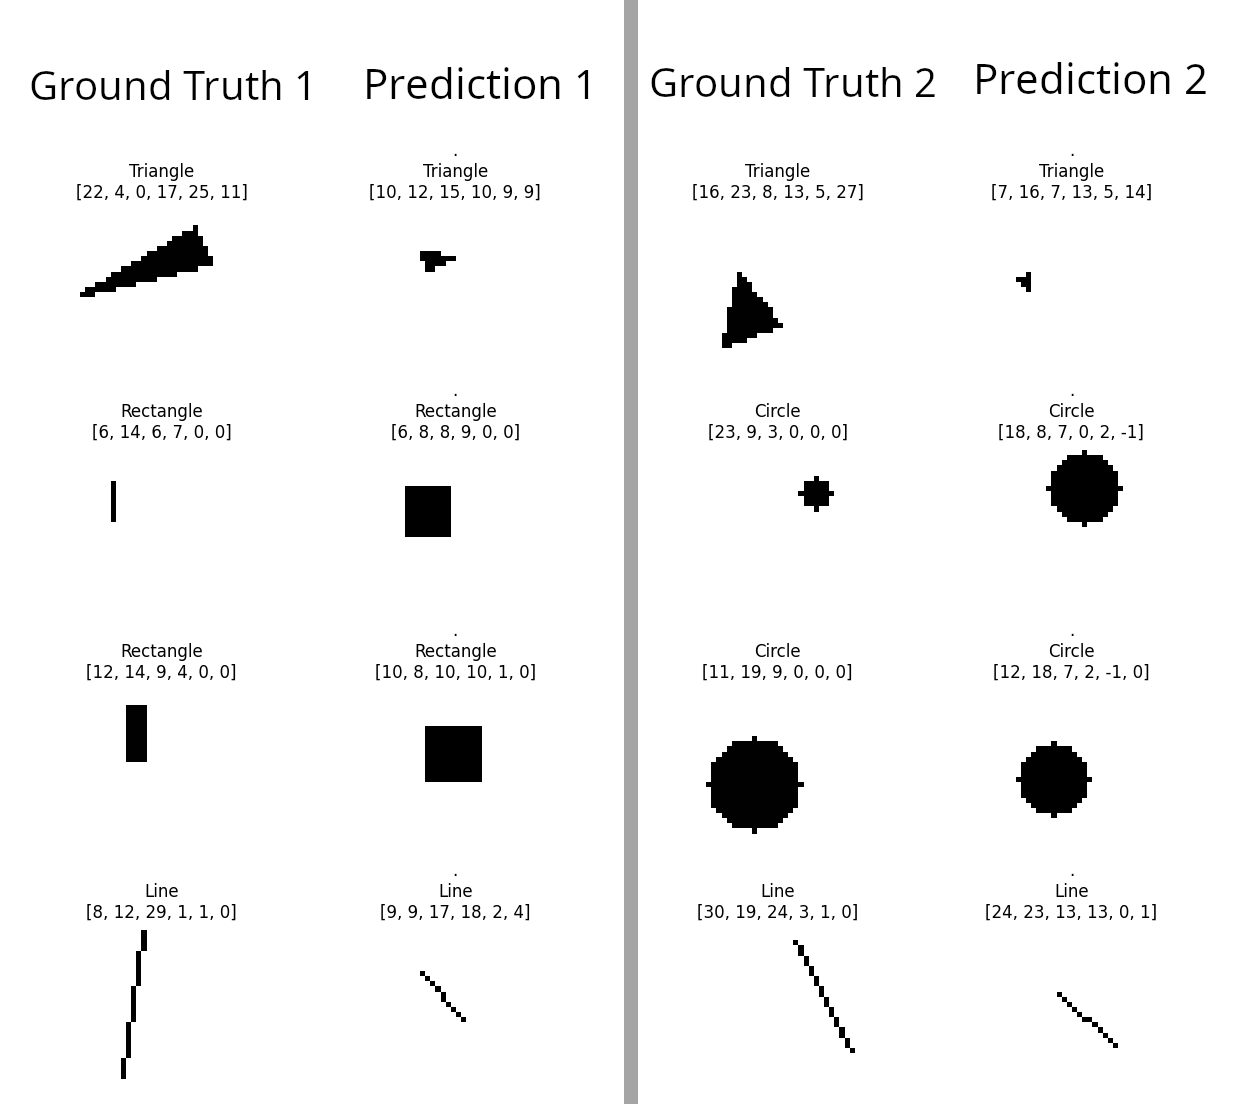
\includegraphics[width=1.0\textwidth]{../rc/images/all_shapes_approx_visual1_condensed.png}
   \label{fig:results_demonstration1}
\end{figure}

\begin{figure}[H]
   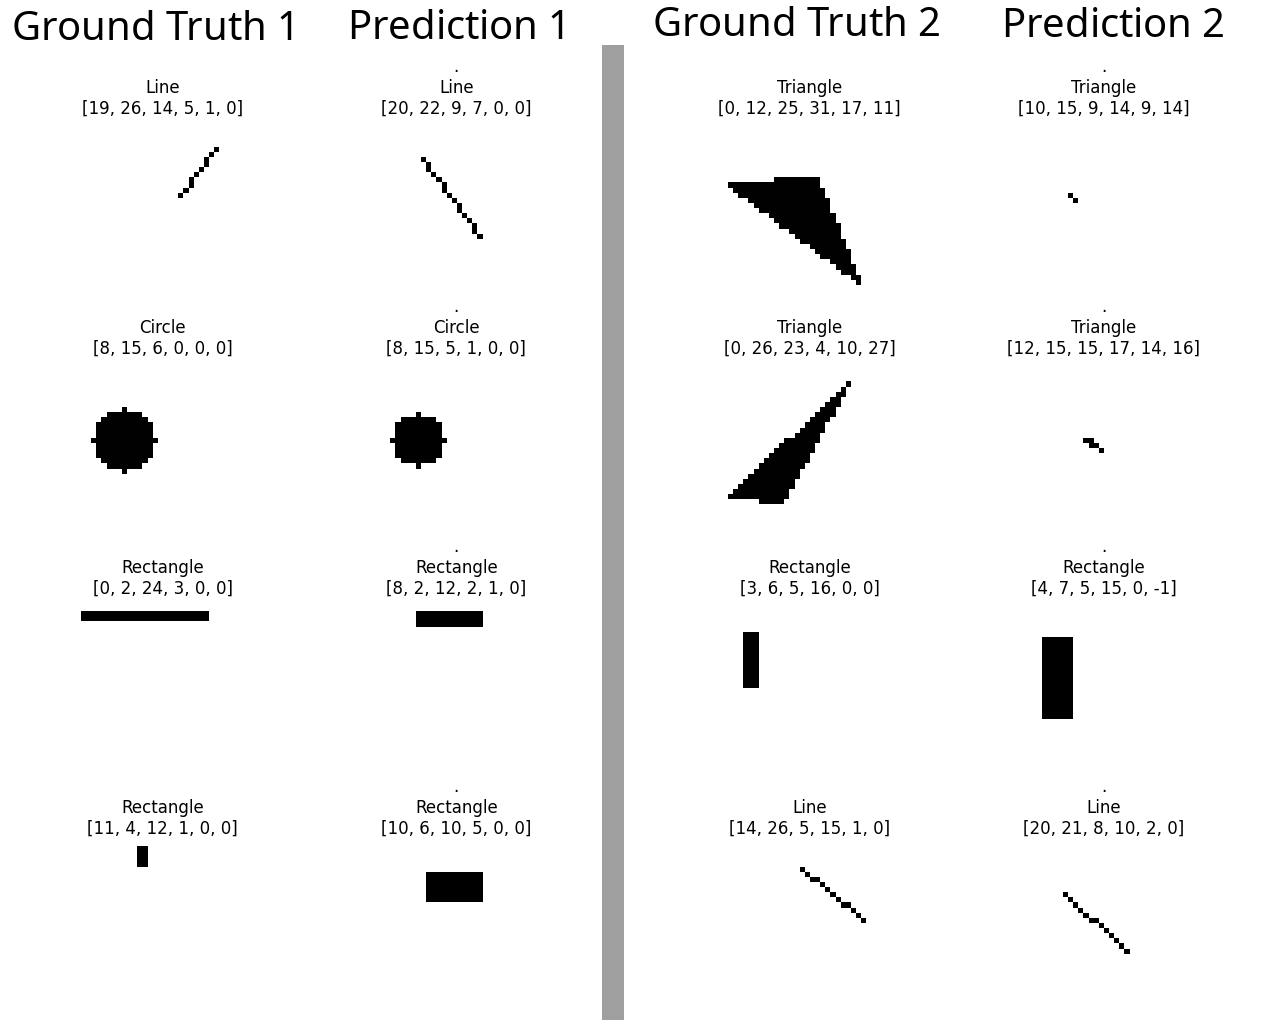
\includegraphics[width=1.0\textwidth]{../rc/images/all_shapes_approx_visual2_condensed.png}
   \label{fig:results_demonstration2}
\end{figure}

\begin{figure}[H]
   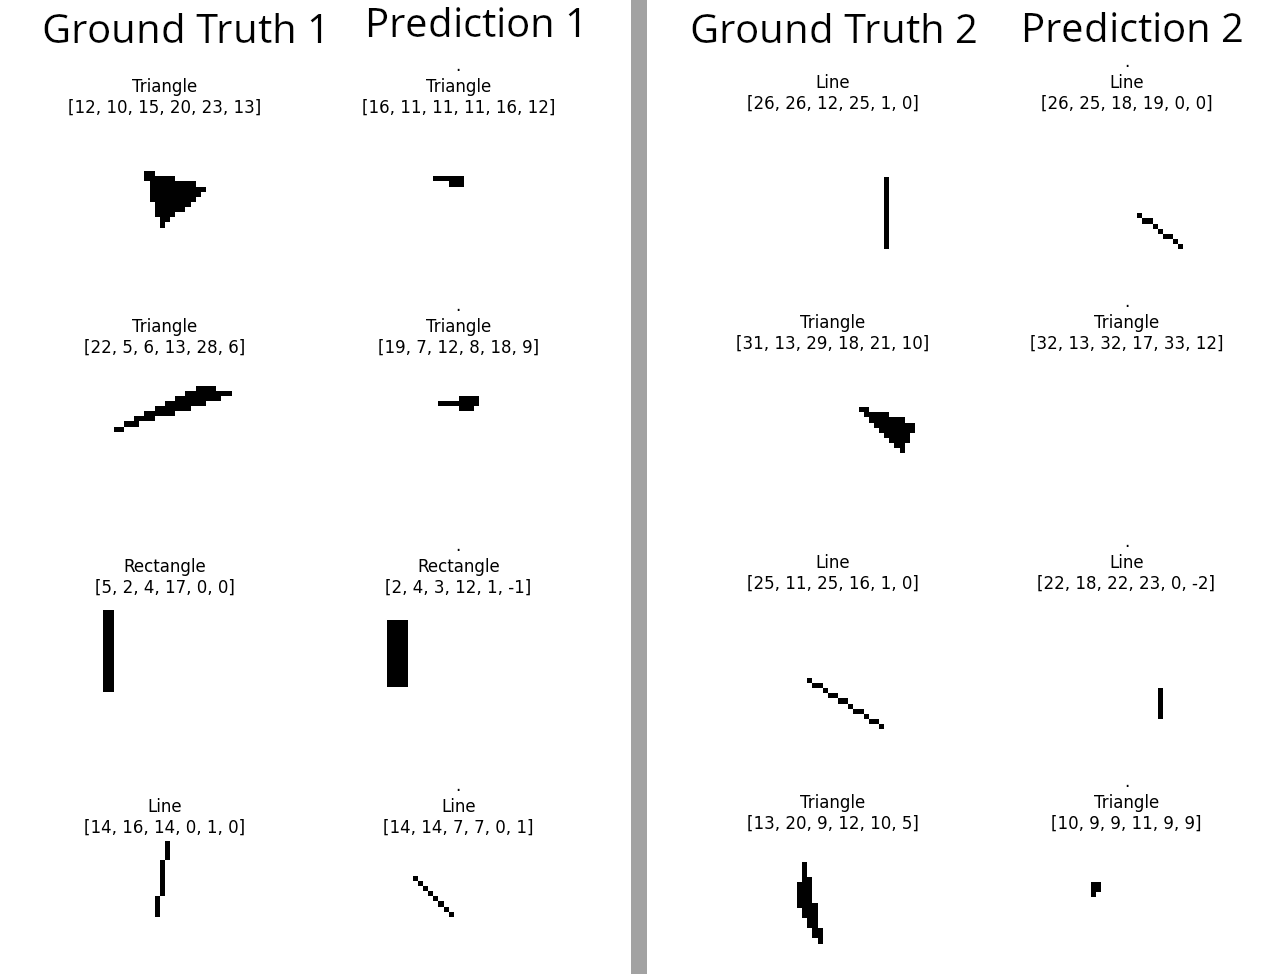
\includegraphics[width=1.0\textwidth]{../rc/images/all_shapes_approx_visual3_condensed.png}
   \label{fig:results_demonstration3}
\end{figure}

%----------------------------------------------%
% }}}
%----------------------------------------------%


%----------------------------------------------%
% {{{
%----------------------------------------------%

\pagebreak

Hiermit bestätige ich, Lars Hösli, meine Maturaarbeit selbstständig verfasst
und alle verwendeten Quellen wahrheitsgetreu angegeben zu haben.

Ich nehme zur Kenntnis, dass meine Arbeit zur Überprüfung der korrekten und
vollständigen Angabe der Quellen mit Hilfe einer Software geprüft wird. Zu meinem
eigenen Schutz wird die Software auch dazu verwendet, später eingereichte Arbeiten mit meiner Arbeit elektronisch zu vergleichen und damit Abschriften und
eine Verletzung meines Urheberrechts zu verhindern. Falls Verdacht besteht, dass
mein Urheberrecht verletzt wurde, erkläre ich mich damit einverstanden, dass die
Schulleitung meine Arbeit zu Prüfzwecken herausgibt.

\vspace{2.0cm}
\emph{Glarus, 03.12.2023}\\
--------------------------------- ------------------------------------

Ort, Datum und Unterschrift

%----------------------------------------------%
% }}}
%----------------------------------------------%


\end{document}
